\documentclass[11pt]{article}
\usepackage[a4paper,margin=1in]{geometry}
\usepackage{booktabs}
\usepackage{enumitem}
\usepackage{hyperref}
\usepackage{graphicx}
\usepackage{tikz}
\usetikzlibrary{arrows.meta,positioning}
\setlist{nosep}
\title{Week 1 Design Report: Urban Data Integration Platform}
\author{Data-Intensive Computing}
\date{}
\begin{document}
\maketitle

\section{Purpose}
This project builds a reusable Spark and Delta Lake platform for four urban datasets: taxi trips, weather, air quality, and taxi zones. The goal is to preserve the source data, validate and standardise it, then create one analytical table in which each taxi trip has contextual weather, air-quality, and zone information. The implementation uses a raw--bronze--silver--gold structure so that errors in a later stage can be corrected without changing the original files.

\section{Data Catalog}
\begin{center}
\small
\begin{tabular}{p{2.2cm}p{2.7cm}p{3.0cm}p{2.8cm}}
\toprule
Dataset & Entity and key & Main join fields & Growth and notes \\
\midrule
Taxi trips & One trip; no reliable natural key & Pickup/dropoff location; pickup hour & Large fact table; grows continuously. A tested composite key was not unique, so no artificial key is used. \\
Weather & One hourly observation; year, month, day, hour & Constructed hourly timestamp & Small reference dataset. \\
Air quality & One site/parameter observation; site, parameter, POC, local date/time & Selected site and hourly timestamp & Large sensor dataset with many sites. \\
Taxi zones & One zone; location ID & Pickup and dropoff location ID & Small lookup table. \\
\bottomrule
\end{tabular}
\end{center}

The key integration risk is air quality. A time-only join would match a trip to many monitoring sites and multiply trip rows. The platform therefore selects one documented NYC site and aggregates only duplicate records from that site within the same hour.

\section{Storage Architecture}
Raw files are kept unchanged in \texttt{data/raw}. Bronze Delta tables apply only necessary column renaming, timestamp parsing, validation, and partition columns. Silver Delta tables apply the common data model. Gold contains \texttt{integrated\_taxi\_trips}; this is the table intended for analysis.

Taxi trips and air quality are partitioned by year and month because they are large and commonly queried by time. Weather and taxi zones are not partitioned: their small size makes partition metadata more expensive than any pruning benefit. At much larger scale, daily partitions and file compaction could be considered, but these add complexity that is not justified by the current data volume.

\section{Common Data Model}
All names use \texttt{snake\_case}. Datetimes use Spark \texttt{timestamp}; categorical identifiers use integer types; numeric measurements use doubles; labels remain strings. Empty columns are dropped. Weather precipitation nulls become zero where domain meaning supports it, while meaningful air-quality qualifier nulls are retained. Air-quality \texttt{date\_local} and \texttt{time\_local} are combined into \texttt{aq\_timestamp}, which supports a valid hourly join.

\section{Ingestion Framework}
The generic pipeline is driven by a configuration entry per dataset. Each entry contains the input path and format, required columns, primary key where available, partitioning choice, and dataset-specific rule. The shared code loads CSV or Parquet, standardises names, validates required columns, parses timestamps, rejects invalid keys, duplicates, and invalid timestamps, writes Delta output, and records row counts and elapsed time in a metadata Delta table.

This design avoids one script per source. Adding a dataset normally means adding configuration and a small rule rather than copying the full ingestion flow. Dataset-specific rules remain configuration-level because a valid taxi distance is a different concept from a valid weather hour.

\clearpage
\section{Integration Strategy}
Trips are enriched in four left joins. Weather joins on pickup hour. Air quality joins on pickup hour after filtering to the selected site and producing one PM2.5 value per hour. The final hourly AQ join matched 8,440,842 of 8,480,870 trips (99.5\%). Taxi zones join twice, once for pickup and once for dropoff. Left joins retain every accepted trip even if an observation is missing. Weather, selected air quality, and zone tables are small enough to broadcast, avoiding a costly shuffle of the taxi fact table.

The principal trade-off is spatial precision versus simplicity. A fixed site is reproducible and prevents row multiplication, but it does not represent the exact air quality at every trip location. Nearest-site matching would be more accurate but adds spatial data and substantially more computation.

\section{Engineering Decisions and Trade-offs}
Delta Lake was selected over plain Parquet because its transaction log provides reliable writes, schema enforcement, and a useful base for later incremental updates. Layered storage favours recoverability and clear responsibility over minimal storage duplication. Configuration-driven ingestion favours maintainability over source-specific optimisation.

The benchmark compares monthly partitioned taxi trips with a flat Delta table. At the current three-month scale, the flat table is marginally faster for full scans because the benchmark queries do not filter by year or month. Partitioning costs more to write and creates more files, but remains the appropriate long-term design for time-filtered queries as the dataset grows.

\section{Architecture Diagram}
\begin{center}
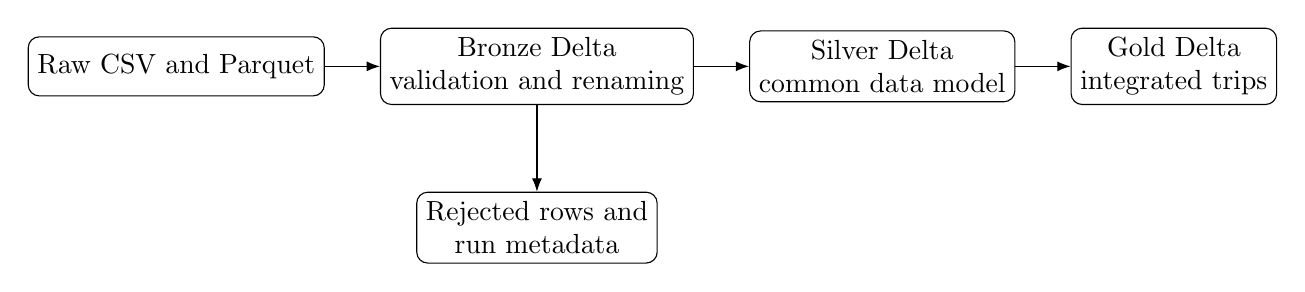
\begin{tikzpicture}[node distance=1.1cm and 0.7cm, every node/.style={draw, rounded corners, align=center, minimum width=2.1cm, minimum height=0.75cm}, >=Latex]
\node (raw) {Raw CSV and Parquet};
\node (bronze) [right=of raw] {Bronze Delta\\validation and renaming};
\node (silver) [right=of bronze] {Silver Delta\\common data model};
\node (gold) [right=of silver] {Gold Delta\\integrated trips};
\node (meta) [below=of bronze] {Rejected rows and\\run metadata};
\draw[->] (raw) -- (bronze);
\draw[->] (bronze) -- (silver);
\draw[->] (silver) -- (gold);
\draw[->] (bronze) -- (meta);
\end{tikzpicture}
\end{center}

\end{document}
